% Options for packages loaded elsewhere
\PassOptionsToPackage{unicode}{hyperref}
\PassOptionsToPackage{hyphens}{url}
%
\documentclass[
  12pt,
]{article}
\usepackage{amsmath,amssymb}
\usepackage{iftex}
\ifPDFTeX
  \usepackage[T1]{fontenc}
  \usepackage[utf8]{inputenc}
  \usepackage{textcomp} % provide euro and other symbols
\else % if luatex or xetex
  \usepackage{unicode-math} % this also loads fontspec
  \defaultfontfeatures{Scale=MatchLowercase}
  \defaultfontfeatures[\rmfamily]{Ligatures=TeX,Scale=1}
\fi
\usepackage{lmodern}
\ifPDFTeX\else
  % xetex/luatex font selection
  \setmainfont[]{Arial}
\fi
% Use upquote if available, for straight quotes in verbatim environments
\IfFileExists{upquote.sty}{\usepackage{upquote}}{}
\IfFileExists{microtype.sty}{% use microtype if available
  \usepackage[]{microtype}
  \UseMicrotypeSet[protrusion]{basicmath} % disable protrusion for tt fonts
}{}
\makeatletter
\@ifundefined{KOMAClassName}{% if non-KOMA class
  \IfFileExists{parskip.sty}{%
    \usepackage{parskip}
  }{% else
    \setlength{\parindent}{0pt}
    \setlength{\parskip}{6pt plus 2pt minus 1pt}}
}{% if KOMA class
  \KOMAoptions{parskip=half}}
\makeatother
\usepackage{xcolor}
\usepackage[margin=1in]{geometry}
\usepackage{graphicx}
\makeatletter
\def\maxwidth{\ifdim\Gin@nat@width>\linewidth\linewidth\else\Gin@nat@width\fi}
\def\maxheight{\ifdim\Gin@nat@height>\textheight\textheight\else\Gin@nat@height\fi}
\makeatother
% Scale images if necessary, so that they will not overflow the page
% margins by default, and it is still possible to overwrite the defaults
% using explicit options in \includegraphics[width, height, ...]{}
\setkeys{Gin}{width=\maxwidth,height=\maxheight,keepaspectratio}
% Set default figure placement to htbp
\makeatletter
\def\fps@figure{htbp}
\makeatother
\setlength{\emergencystretch}{3em} % prevent overfull lines
\providecommand{\tightlist}{%
  \setlength{\itemsep}{0pt}\setlength{\parskip}{0pt}}
\setcounter{secnumdepth}{-\maxdimen} % remove section numbering
\ifLuaTeX
  \usepackage{selnolig}  % disable illegal ligatures
\fi
\usepackage{bookmark}
\IfFileExists{xurl.sty}{\usepackage{xurl}}{} % add URL line breaks if available
\urlstyle{same}
\hypersetup{
  pdfauthor={Nick Xing; Zihan Zhu; Noah Clark},
  hidelinks,
  pdfcreator={LaTeX via pandoc}}

\title{Hospital Insurance Charges Model \vspace{0.5cm}\\
Final for STAT 425}
\author{Nick Xing \and Zihan Zhu \and Noah Clark}
\date{May 6, 2024}

\begin{document}
\maketitle

{
\setcounter{tocdepth}{3}
\tableofcontents
}
\newpage

\subsection{Section 1: Introduction}\label{section-1-introduction}

This project focuses on the analysis of medical insurance data,
particularly focusing on the medical charges acquired from hospital
visits. The response variable is the variable charges from the insurance
data. This data is found on Kaggle, as was last updated 6 years ago, in
2018. In this data set, there 6 variables excluding the response
variable, charges, which shows the exact charges the patient acquired
from their hospital visit. Each variable is defined within the Kaggle
(2018) website and explained in this order:

\begin{itemize}
\item
  age: age of primary beneficiary
\item
  sex: insurance contractor gender, female, male
\item
  bmi: Body mass index, providing an understanding of body, weights that
  are relatively high or low relative to height, objective index of body
  weight (kg / m \^{} 2) using the ratio of height to weight, ideally
  18.5 to 24.9
\item
  children: Number of children covered by health insurance / Number of
  dependents
\item
  smoker: Smoking
\item
  region: the beneficiary's residential area in the US, northeast,
  southeast, southwest, northwest.
\item
  charges: Individual medical costs billed by health insurance

  This report compares multiple models derived from analysis of the data
  set including an Explanatory Model, a Linear Regression Model, a
  Regression Tree, and a Random Forest. All analyses are performed in
  the R environment. This is possible to recreate with the code provided
  in this file. Setting seeds might yield slightly different results;
  however, we did not use a seed to analyze this data. No function
  (i.e.~\emph{set.seed}) should change the results concluded from this
  data, although it is possible to slightly alter the data using said
  functions. Again, the results would be concluded the same way. This
  report has 4 sections. Section 1 is this introduction. Section 2 uses
  modelling assumptions and models to analyze the data and provide
  insights on the data. Section 3 presents predictive models and shows
  training from said models. Section 4 compares models and provides a
  discussion of these results.
\end{itemize}

\newpage

\subsection{Section 2: Exploratory Data
Analysis}\label{section-2-exploratory-data-analysis}

Here is a brief overview of all of the variables of this dataset:

Numerical Variables:

\begin{itemize}
\tightlist
\item
  age: age of primary beneficiary
\item
  bmi: body mass index
\item
  children: number of children/dependents covered by health insurance
\item
  charges (response variable): medical costs billed by health insurance
\end{itemize}

Categorical Variables:

\begin{itemize}
\tightlist
\item
  sex: male or female
\item
  smoker: yes or no
\item
  region: residential area in the US, can be northeast, southeast,
  southwest, or northwest
\end{itemize}

The first step is to check for unusual observations by performing an
outlier test. To do so, we obtained the studentized residuals for our
data, and compared the largest values with the Bonferroni critical
value.

This is the Bonferroni critical value we calculated:

\begin{verbatim}
## [1] -4.137174
\end{verbatim}

Next, here are the five largest studentized residuals, which we will be
comparing to the Bonferroni critical value:

\begin{verbatim}
##     1301      578      243      220      517 
## 5.009599 4.219800 4.053228 3.998326 3.863878
\end{verbatim}

Since the absolute value of their respective studentized residual is
greater than the Bonferroni critical value, we can conclude that
Observation \#1301 and Observation \#578 are outliers.

We also checked Cook's distance, however we found that there is no point
with Cook's distance greater than 1. We will simply remove the two
outliers we found earlier.

\newpage

After removing these two points, we will be analyzing the predictors to
see if there are any variables we should add or remove.

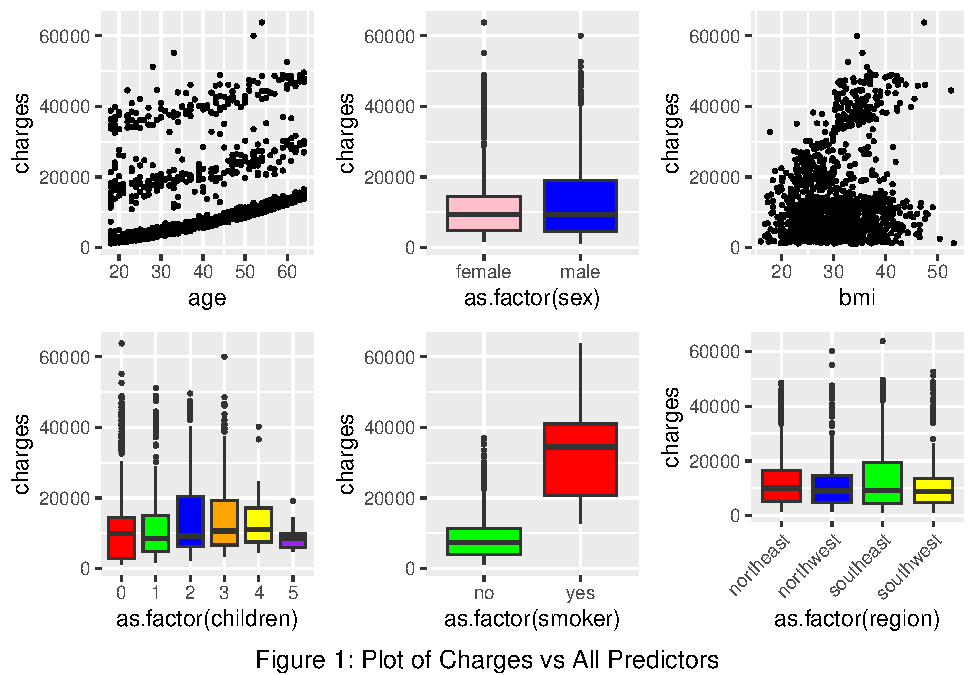
\includegraphics{finalproject_files/figure-latex/unnamed-chunk-7-1.pdf}

From the plot of charges vs age, we notice a trend that the charges
increase as age increases. We will not be removing `age' as a predictor
since it is clear that it has a significant impact on the response
variable `charges'. This makes sense because as people grow older, their
health declines, and the insurance costs increase.

The charges vs sex boxplot tells us that males tend to have higher
charges than females. We will conduct a t-test to test this difference.

We obtained this p-value from the t-test:

\begin{verbatim}
## $p.value
## [1] 0.03460436
\end{verbatim}

Given that the p-value is less than 0.05, we conclude that `sex' is a
significant predictor, with males incurring higher insurance costs than
females. A possible explanation for this is that males are usually more
at risk of health conditions that result in increased charges compared
to females.

From the plot of charges vs bmi, we can see a general trend that as bmi
increases, the charges also increase. As a result, we will not be
removing `bmi' as a predictor since it appears to have an impact on the
response variable. The graph also makes sense logically since people
with a higher bmi tend to be overweight and subsequently, have worse
health than people with a lower bmi, causing their insurance charges to
be greater as well.

The boxplot of charges vs children conveys to us that charges tend to
increase as the number of children grows from 0 or 1 to 2 or 3. While
there are some data points for people with 4 or 5 children, it appears
that these groups have a very low amount of people, and it may be
challenging to draw meaningful conclusions from it. We perform an ANOVA
test to test the significance of `children' as a predictor.

This is the p-value we obtain:

\begin{verbatim}
## [1] 0.008620164
\end{verbatim}

This p-value is less than 0.05, thus signifying that the predictor
`children' is significant. We will be keeping as a predictor in our
model. A larger number of children/dependents covered leads to higher
charges, as there are more individuals who need to be covered.

From the boxplot of charges vs smoker, it is evident that smokers
generally face significantly higher charges than non-smokers.
Consequently, we will not be removing `smoker' as a predictor. People
who smoke typically incur higher insurance costs due to the health risks
posed by smoking.

The boxplot of charges vs region shows us that the southeast region
seemingly has higher charges than the other three regions. We will
conduct an ANOVA test to make sure that the predictor `region' is
significant.

This is the p-value we obtained from the ANOVA test:

\begin{verbatim}
## [1] 0.04525914
\end{verbatim}

The p-value is less than 0.05, indicating that the predictor `region' is
significant, and thus we will retain it as a predictor. This confirms
that there are regional differences in the insurance costs.

\newpage

Now, we will explore whether or not we should include any interactions
between categorical variables. We will be analyzing all possible
first-order and second-order interactions between our categorical
predictors, including:

\begin{itemize}
\tightlist
\item
  `sex' and `smoker'
\item
  `sex' and `region'
\item
  `region' and `smoker'
\item
  `sex', `smoker', and `region'
\end{itemize}

Here are some plots that show the interactions between these predictors.

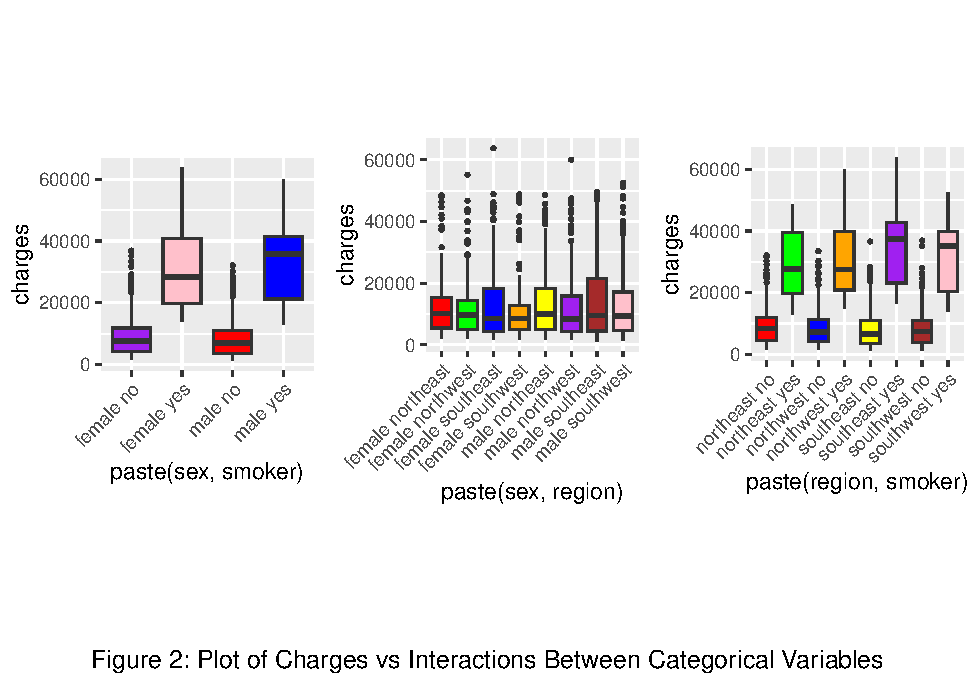
\includegraphics{finalproject_files/figure-latex/unnamed-chunk-11-1.pdf}

From the plots, it appears as though smoking increases the charges more
for males than females. Additionally, it seems like smoking has a
greater impact on charges in the southeast and southwest, when compared
to northeast and northwest. However, it does not appear that sex and
region is a significant interaction.

We applied sequential F-tests with the anova function to assess the
significance of the interaction terms in our model. Initially, we
included all potential interactions among the three variables `sex',
`smoker', and `region'. We first found that the second-order interaction
sex:smoker:region was not significant, and removed it from the model.
Subsequently, we tested the first-order interactions and found that the
interaction sex:region was not significant. Finally, after removing
sex:region as a predictor, we concluded that only the interactions
sex:smoker and smoker:region are statistically significant, and we will
retain them in the final model.

\newpage

Now, we will examine the numerical variables and see if there is
evidence of any nonlinear trends.

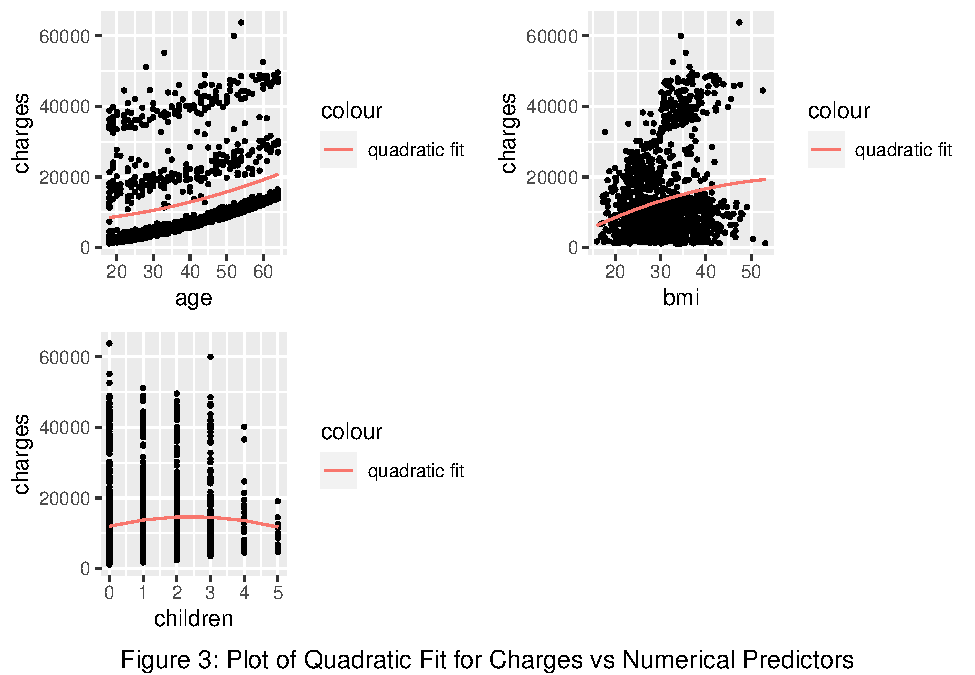
\includegraphics{finalproject_files/figure-latex/unnamed-chunk-16-1.pdf}

Based on the plot of the quadratic fit for charges vs age, we see there
is evidence of non-linearity for the predictor `age' since the quadratic
fit has some upward curvature.

Similarly, based on the plot of the quadratic fit for charges vs bmi, we
see there is some evidence of non-linearity for the predictor `bmi',
although maybe not as clear as for `age'. This time, the quadratic fit
curves downwards.

Finally, the plot of charges vs children also suggests some
non-linearity. However, the non-linearity is not as evident as for `age
and 'bmi' since although the quadratic fit does appear to curve
downwards as the number of children increases, there is not many data
points for 4 and 5 children, so we may not be able to draw a strong
conclusion.

\newpage

\subsection{Section 3: Methodology}\label{section-3-methodology}

You are required to build at least two prediction models using the
methods covered in this class. For each model or method you are using,
include a brief description of the methodology and a description of the
R implementation (R coding steps).

Your should consider the following sub-sections: Section 3.1: Start with
a simple model, a model that doesn't require much training, for example,
a linear regression model built after appropriate variable selection and
model diagnostics. Section 3.2: Use the Linear Regression model built in
1 to make predictions on a testing set. Section 3.3: Fit a different
kind of model like a non-parametric regression, regularized regression
models or others, and make a prediction on the same testing set. Section
3.4 (Optional): You can also try with other methods learnt in other
classes if applicable (like for example Random Forests).

\newpage

\subsection{Section 4: Discussion and
Conclusions}\label{section-4-discussion-and-conclusions}

In this part you should make a summary of your results by comparing the
different modeling approaches and discussing the impact of your
analysis. You should also write the main conclusions of your analysis in
three to four bullet points.

\end{document}
